% Module 6: AI Hardware and Acceleration - Short Assignment
% Compile with XeLaTeX: latexmk -xelatex report.tex
\documentclass{article}

\PassOptionsToPackage{numbers,compress}{natbib}
\usepackage[final]{template22}
% Common packages and layout for the Module 6 short report.
\usepackage[T1]{fontenc}
\usepackage{microtype}
\usepackage{times}
\usepackage{graphicx}
\usepackage{amsmath,amssymb}
\usepackage{enumitem}
\usepackage{booktabs,tabularx,array}
\usepackage[skip=3pt,font=small]{caption}
\usepackage[pagebackref=true,breaklinks=true,colorlinks]{hyperref}
\usepackage{xspace}

\hypersetup{
  pdfencoding=auto,
  colorlinks=true,
  allcolors=black
}

\usepackage{fancyhdr}
\renewcommand{\headrulewidth}{0.5pt}
\renewcommand{\footrulewidth}{0pt}
\fancyhf{}
\fancyfoot[C]{\thepage}

\setlength{\floatsep}{0.5\baselineskip plus 3pt minus 2pt}
\setlength{\textfloatsep}{0.5\baselineskip plus 3pt minus 2pt}
\graphicspath{{figures/}}

\newcommand{\numpy}{\textsc{NumPy}\xspace}
\newcommand{\pytorch}{\textsc{PyTorch}\xspace}


\title{CPU and GPU Matrix Multiplication in NumPy and PyTorch}

\author{%
  Yuanze Lei \quad 2510124204\\
  Peking University
}

\begin{document}
\maketitle

\begin{abstract}
This short study compares three matrix-multiplication methods on identical
inputs: NumPy CPU, PyTorch CPU, and PyTorch CUDA. We measure five matrix sizes
and three tensor ranks on an AMD Ryzen 7 5800H and an NVIDIA RTX 3050 Ti.
PyTorch CPU has its largest advantage near size 128, but it approaches NumPy at
size 1024. CUDA carries a clear launch and synchronization cost at sizes 64 and
128; after the crossover near 256, it becomes decisively faster. At size 1024,
CUDA is 9.57x to 13.78x faster than NumPy across the three ranks. We relate the
curves to the CPU BLAS path and the GPU cuBLAS, SM, tiling, and memory path.
\end{abstract}

\section{Scope and Setup}\label{sec:scope}

All three methods compute the same \texttt{float32} products with fixed random
seeds. NumPy CPU \citep{harris2020numpy} uses OpenBLAS \citep{openblas};
PyTorch CPU \citep{paszke2019pytorch} uses MKL; PyTorch CUDA uses the GPU. The
CPU runs use eight threads. CUDA inputs are copied to the GPU before timing, so
the GPU result measures launch, output allocation, kernel execution, and
completion, but excludes host-to-device transfer. This isolates the
repeated-compute case where data already reside on the accelerator.

\begin{center}
\captionof{table}{Measured environment and timing controls.}
\label{tab:environment}
\small
\begin{tabularx}{\linewidth}{@{}lX@{}}
\toprule
CPU & AMD Ryzen 7 5800H, 8 cores / 16 threads, 8 threads used \\
GPU & NVIDIA RTX 3050 Ti Laptop, 20 SMs, 4 GiB, compute capability 8.6 \\
Software & Python 3.14.4, NumPy 2.4.4, PyTorch 2.12.0, CUDA 12.6 \\
Precision & IEEE FP32; PyTorch TF32 disabled in this run \\
GPU timing & \texttt{perf\_counter} plus \texttt{cuda.synchronize} \\
Repeats & warm-up 5; median of 9--50 interleaved calls \\
\bottomrule
\end{tabularx}
\end{center}

\subsection{Workloads and protocol}

For side length $s$, the benchmark uses the matched shapes
\begin{equation}\label{eq:shapes}
\begin{aligned}
\text{2D:}\quad &(\mathbf A,\mathbf B)\in\mathbb R^{s\times s}
  \times \mathbb R^{s\times s},\\
\text{3D:}\quad &(\mathbf A,\mathbf B)\in\mathbb R^{4\times s\times s}
  \times \mathbb R^{4\times s\times s},\\
\text{4D:}\quad &(\mathbf A,\mathbf B)\in\mathbb R^{2\times 2\times s\times s}
  \times \mathbb R^{2\times 2\times s\times s}.
\end{aligned}
\end{equation}
The sizes are $s\in\{64,128,256,512,1024\}$. Rank-3 and rank-4 cases both
contain four matrix products, so they compare indexing dimension at nearly
constant work. We verify CPU and CUDA outputs against NumPy with
$\mathrm{rtol}=\mathrm{atol}=10^{-4}$.

The timed operations are \texttt{np.matmul}, CPU \texttt{torch.matmul}, and
CUDA \texttt{torch.matmul}. Method order rotates between repetitions to reduce
cache or frequency bias. The stored time is the median in seconds. Speedup is
$S=t_{\mathrm{reference}}/t_{\mathrm{method}}$; values above one favor the
denominator.

\section{Three-Method Results}\label{sec:results}

Figure~\ref{fig:timing} shows the absolute times and Table~\ref{tab:results}
lists every measurement. The two CPU curves are close at large sizes. At
$s=1024$, PyTorch CPU is only 1.02x, 1.01x, and 1.05x faster than NumPy for
2D, 3D, and 4D. Their largest gap is near 128, where PyTorch CPU is
2.55x--3.84x faster in this environment.

\begin{figure}[t]
  \centering
  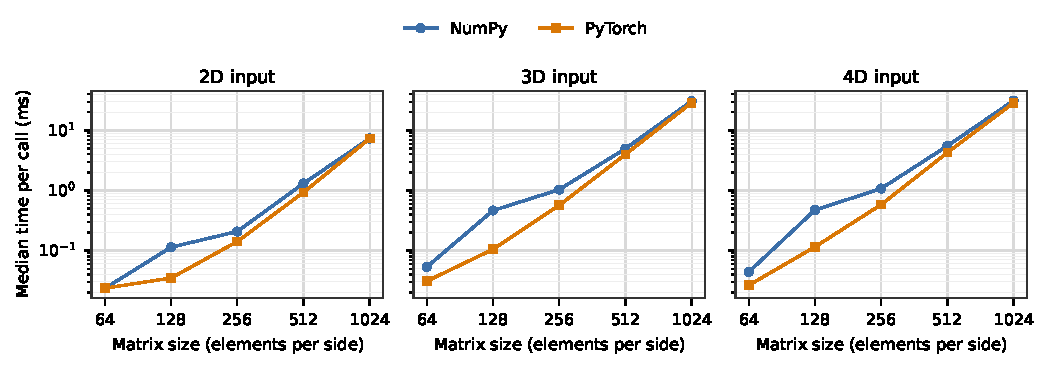
\includegraphics[width=\linewidth]{timing_by_rank.pdf}
  \caption{Median call time for the three methods. Both axes are logarithmic.
  CUDA has nearly flat launch-dominated cost at small sizes and pulls away
  once matrix work is large enough.}
  \label{fig:timing}
\end{figure}

\begin{table}[t]
\caption{Measured median time in milliseconds. $S_{\mathrm{cpu}}$ compares
PyTorch CPU with NumPy; $S_{\mathrm{gpu}}$ compares PyTorch CUDA with NumPy.}
\label{tab:results}
\centering
\scriptsize
\setlength{\tabcolsep}{4.2pt}
\begin{tabular}{@{}rrrrrrr@{}}
\toprule
Rank & $s$ & NumPy & Torch CPU & Torch CUDA & $S_{\mathrm{cpu}}$ & $S_{\mathrm{gpu}}$ \\
\midrule
2D & 64   & 0.0213 & 0.0312 & 0.0835 & 0.68 & 0.25 \\
2D & 128  & 0.1451 & 0.0568 & 0.1117 & 2.55 & 1.30 \\
2D & 256  & 0.2624 & 0.1615 & 0.1232 & 1.62 & 2.13 \\
2D & 512  & 1.3395 & 1.0357 & 0.2882 & 1.29 & 4.65 \\
2D & 1024 & 7.4834 & 7.3206 & 0.7822 & 1.02 & 9.57 \\
\midrule
3D & 64   & 0.0724 & 0.0707 & 0.1657 & 1.02 & 0.44 \\
3D & 128  & 0.5230 & 0.1451 & 0.2149 & 3.60 & 2.43 \\
3D & 256  & 1.1857 & 0.6512 & 0.2722 & 1.82 & 4.36 \\
3D & 512  & 5.3887 & 4.2720 & 0.6135 & 1.26 & 8.78 \\
3D & 1024 & 31.2711 & 31.0720 & 2.4242 & 1.01 & 12.90 \\
\midrule
4D & 64   & 0.0712 & 0.0827 & 0.1698 & 0.86 & 0.42 \\
4D & 128  & 0.5634 & 0.1467 & 0.1774 & 3.84 & 3.17 \\
4D & 256  & 1.2474 & 0.7071 & 0.3391 & 1.76 & 3.68 \\
4D & 512  & 5.5868 & 4.2406 & 0.6068 & 1.32 & 9.21 \\
4D & 1024 & 30.4119 & 28.9698 & 2.2076 & 1.05 & 13.78 \\
\bottomrule
\end{tabular}
\end{table}

\begin{figure}[t]
  \centering
  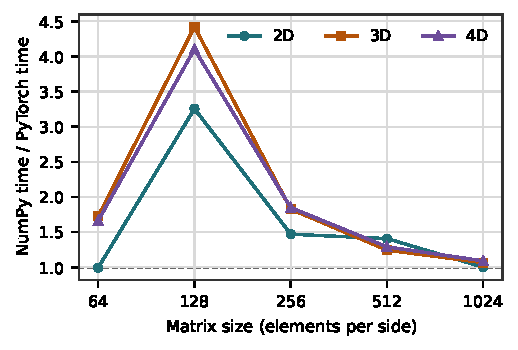
\includegraphics[width=\linewidth]{speedup_by_rank.pdf}
  \caption{Three direct comparisons. Left: NumPy versus PyTorch CPU. Middle:
  NumPy versus PyTorch CUDA. Right: PyTorch CPU versus CUDA. The dashed line
  marks parity. All vertical axes are logarithmic.}
  \label{fig:speedup}
\end{figure}

\subsection{GPU crossover and scaling}

Figure~\ref{fig:speedup} exposes the crossover. At $s=64$, CUDA takes
0.0835--0.1698 ms, so launch and synchronization overhead dominate. PyTorch CPU
is 2.7x, 2.3x, and 2.1x faster than CUDA in the three ranks. At $s=256$, CUDA
has overtaken PyTorch CPU for every rank. At $s=1024$, PyTorch CPU/CUDA
speedups are 9.36x, 12.82x, and 13.12x.

The batched ranks scale better than 2D. Four matrix products expose more
parallel tiles to the 20 SMs. Rank-3 and rank-4 curves nearly coincide because
they execute the same four products; flattening the batch is not the dominant
cost. The 2D case has less parallel work and therefore a lower CUDA/CPU
speedup at 1024.

\section{Why the Paths Differ}\label{sec:principles}

\subsection{CPU: two BLAS paths}

Neither CPU call performs a Python-level triple loop. NumPy dispatches to
OpenBLAS, while PyTorch CPU dispatches to a compiled MKL-enabled path. Both use
kernels that tile the matrices so a block remains in cache while many
multiply-add operations are accumulated. They then vectorize with SIMD and
distribute blocks across the eight CPU threads. The observed difference is
mainly the dispatch and BLAS implementation, not NumPy arrays versus PyTorch
tensors as containers. At large sizes both become limited by the same DRAM
traffic and available CPU cores, which explains their convergence.

\subsection{GPU: launch, SM tiling, and memory}

For CUDA, the Python caller reaches PyTorch's dispatcher, which launches a
cuBLAS GEMM kernel \citep{nvidia2026cublas}. The CPU does not execute the
multiply-add loop. The GPU schedules blocks of work on its 20 streaming
multiprocessors (SMs). Threads load input tiles from GPU memory into shared
memory or registers, reuse those tiles for several products, and write the
output tile back to GPU memory. Many warps overlap arithmetic with memory
latency \citep{nvidia2026cuda}. A rank-3 or rank-4 input becomes a batch of
GEMMs, giving the scheduler more independent blocks.

This path has two fixed costs: launching the kernel and synchronizing the CPU
with completion. They are small in absolute terms but dominate a 64 or 128
problem. Once each GEMM contains enough work, thousands of active threads and
high GPU memory bandwidth outweigh those costs. TF32 was disabled, so the
result does not depend on tensor-core reduced-precision execution.

\section{Limitations and Conclusion}\label{sec:conclusion}

The GPU numbers exclude PCIe transfer and use one laptop GPU. A one-off call
would also pay the transfer cost, so resident data are the favorable but
realistic case for repeated multiplication. Different BLAS libraries, clocks,
or GPU architectures can move the crossover.

The three-method experiment still gives a stable practical conclusion.
PyTorch CPU is useful around medium matrices but converges toward NumPy at
large sizes. CUDA loses on launch overhead below roughly 256 and then scales
strongly with matrix work, reaching 9.57x--13.78x over NumPy at 1024. The
curves follow the expected CPU BLAS and GPU SM/cuBLAS execution models.

\begingroup
\small
\setlength{\bibsep}{2pt}
\bibliographystyle{plainnat}
\bibliography{reference}
\endgroup

\end{document}
